\documentclass[]{elsarticle} %review=doublespace preprint=single 5p=2 column
%%% Begin My package additions %%%%%%%%%%%%%%%%%%%
\usepackage[hyphens]{url}

  \journal{Journal of Transport \& Health} % Sets Journal name


\usepackage{lineno} % add
\providecommand{\tightlist}{%
  \setlength{\itemsep}{0pt}\setlength{\parskip}{0pt}}

\usepackage{graphicx}
\usepackage{booktabs} % book-quality tables
%%%%%%%%%%%%%%%% end my additions to header

\usepackage[T1]{fontenc}
\usepackage{lmodern}
\usepackage{amssymb,amsmath}
\usepackage{ifxetex,ifluatex}
\usepackage{fixltx2e} % provides \textsubscript
% use upquote if available, for straight quotes in verbatim environments
\IfFileExists{upquote.sty}{\usepackage{upquote}}{}
\ifnum 0\ifxetex 1\fi\ifluatex 1\fi=0 % if pdftex
  \usepackage[utf8]{inputenc}
\else % if luatex or xelatex
  \usepackage{fontspec}
  \ifxetex
    \usepackage{xltxtra,xunicode}
  \fi
  \defaultfontfeatures{Mapping=tex-text,Scale=MatchLowercase}
  \newcommand{\euro}{€}
\fi
% use microtype if available
\IfFileExists{microtype.sty}{\usepackage{microtype}}{}
\bibliographystyle{elsarticle-harv}
\usepackage{color}
\usepackage{fancyvrb}
\newcommand{\VerbBar}{|}
\newcommand{\VERB}{\Verb[commandchars=\\\{\}]}
\DefineVerbatimEnvironment{Highlighting}{Verbatim}{commandchars=\\\{\}}
% Add ',fontsize=\small' for more characters per line
\usepackage{framed}
\definecolor{shadecolor}{RGB}{248,248,248}
\newenvironment{Shaded}{\begin{snugshade}}{\end{snugshade}}
\newcommand{\AlertTok}[1]{\textcolor[rgb]{0.94,0.16,0.16}{#1}}
\newcommand{\AnnotationTok}[1]{\textcolor[rgb]{0.56,0.35,0.01}{\textbf{\textit{#1}}}}
\newcommand{\AttributeTok}[1]{\textcolor[rgb]{0.77,0.63,0.00}{#1}}
\newcommand{\BaseNTok}[1]{\textcolor[rgb]{0.00,0.00,0.81}{#1}}
\newcommand{\BuiltInTok}[1]{#1}
\newcommand{\CharTok}[1]{\textcolor[rgb]{0.31,0.60,0.02}{#1}}
\newcommand{\CommentTok}[1]{\textcolor[rgb]{0.56,0.35,0.01}{\textit{#1}}}
\newcommand{\CommentVarTok}[1]{\textcolor[rgb]{0.56,0.35,0.01}{\textbf{\textit{#1}}}}
\newcommand{\ConstantTok}[1]{\textcolor[rgb]{0.00,0.00,0.00}{#1}}
\newcommand{\ControlFlowTok}[1]{\textcolor[rgb]{0.13,0.29,0.53}{\textbf{#1}}}
\newcommand{\DataTypeTok}[1]{\textcolor[rgb]{0.13,0.29,0.53}{#1}}
\newcommand{\DecValTok}[1]{\textcolor[rgb]{0.00,0.00,0.81}{#1}}
\newcommand{\DocumentationTok}[1]{\textcolor[rgb]{0.56,0.35,0.01}{\textbf{\textit{#1}}}}
\newcommand{\ErrorTok}[1]{\textcolor[rgb]{0.64,0.00,0.00}{\textbf{#1}}}
\newcommand{\ExtensionTok}[1]{#1}
\newcommand{\FloatTok}[1]{\textcolor[rgb]{0.00,0.00,0.81}{#1}}
\newcommand{\FunctionTok}[1]{\textcolor[rgb]{0.00,0.00,0.00}{#1}}
\newcommand{\ImportTok}[1]{#1}
\newcommand{\InformationTok}[1]{\textcolor[rgb]{0.56,0.35,0.01}{\textbf{\textit{#1}}}}
\newcommand{\KeywordTok}[1]{\textcolor[rgb]{0.13,0.29,0.53}{\textbf{#1}}}
\newcommand{\NormalTok}[1]{#1}
\newcommand{\OperatorTok}[1]{\textcolor[rgb]{0.81,0.36,0.00}{\textbf{#1}}}
\newcommand{\OtherTok}[1]{\textcolor[rgb]{0.56,0.35,0.01}{#1}}
\newcommand{\PreprocessorTok}[1]{\textcolor[rgb]{0.56,0.35,0.01}{\textit{#1}}}
\newcommand{\RegionMarkerTok}[1]{#1}
\newcommand{\SpecialCharTok}[1]{\textcolor[rgb]{0.00,0.00,0.00}{#1}}
\newcommand{\SpecialStringTok}[1]{\textcolor[rgb]{0.31,0.60,0.02}{#1}}
\newcommand{\StringTok}[1]{\textcolor[rgb]{0.31,0.60,0.02}{#1}}
\newcommand{\VariableTok}[1]{\textcolor[rgb]{0.00,0.00,0.00}{#1}}
\newcommand{\VerbatimStringTok}[1]{\textcolor[rgb]{0.31,0.60,0.02}{#1}}
\newcommand{\WarningTok}[1]{\textcolor[rgb]{0.56,0.35,0.01}{\textbf{\textit{#1}}}}
\usepackage{graphicx}
\ifxetex
  \usepackage[setpagesize=false, % page size defined by xetex
              unicode=false, % unicode breaks when used with xetex
              xetex]{hyperref}
\else
  \usepackage[unicode=true]{hyperref}
\fi
\hypersetup{breaklinks=true,
            bookmarks=true,
            pdfauthor={},
            pdftitle={How do school travel planning stakeholders frame active school travel in Ontario, Canada?},
            colorlinks=false,
            urlcolor=blue,
            linkcolor=magenta,
            pdfborder={0 0 0}}
\urlstyle{same}  % don't use monospace font for urls

\setcounter{secnumdepth}{0}
% Pandoc toggle for numbering sections (defaults to be off)
\setcounter{secnumdepth}{0}

% Pandoc citation processing

% Pandoc header
\usepackage{booktabs}
\usepackage{longtable}
\usepackage{array}
\usepackage{multirow}
\usepackage{wrapfig}
\usepackage{float}
\usepackage{colortbl}
\usepackage{pdflscape}
\usepackage{tabu}
\usepackage{threeparttable}
\usepackage{threeparttablex}
\usepackage[normalem]{ulem}
\usepackage{makecell}
\usepackage{xcolor}



\begin{document}
\begin{frontmatter}

  \title{How do school travel planning stakeholders frame active school travel in
Ontario, Canada?}
    \author[Some Department]{Author 1\corref{1}}
   \ead{author1@example.com} 
    \author[Some Department]{Author 2}
   \ead{author2@example.com} 
    \author[Another University]{Author 3\corref{2}}
   \ead{author3@example.com} 
    \author[Some Institute]{Author 4\corref{2}}
   \ead{author4@example.com} 
    \author[Some University]{Author 5}
   \ead{author5@example.com} 
    \author[Some Department]{Author 6}
   \ead{author6@example.com} 
      \address[Some Department]{Department, Street, City, Province, Postal Code}
    \address[Another University]{Department, Street, City, Province, Postal Code}
    \address[Some Institute]{Street, City, Province, Postal Code}
    \address[Some University]{Department, Street, City, Province, Postal Code}
      \cortext[1]{Corresponding Author}
    \cortext[2]{Equal contribution}
  
  \begin{abstract}
  This is the abstract.
  
  It consists of two paragraphs.
  \end{abstract}
  
 \end{frontmatter}

\textbf{\emph{Background}}:\\
\textbf{\emph{Methods}}:\\
\textbf{\emph{Results}}: \textbf{\emph{Conclusions}}:

\newpage

\hypertarget{introduction}{%
\section{1. Introduction}\label{introduction}}

\hypertarget{school-travel-planning-in-canada}{%
\subsection{1.1. School travel planning in
Canada}\label{school-travel-planning-in-canada}}

Walking and bicycling to school, commonly known as active school travel
or active school transportation (AST), has been declining in Canada and
North America for decades ({\textbf{???}}), with levels much lower than
other developed countries like The Netherlands ({\textbf{???}}) and
Japan ({\textbf{???}}). This trend has prompted a multi-sector response
to identify strategies to increase AST, the most popular of which is a
growing interest in school travel planning across Canada.

School travel planning (STP) is a ``school-specific'' intervention led
by a facilitator that brings together a committee of stakeholders from
diverse sectors including education, planning, transportation, and
public health ({\textbf{???}}). Parents and parent councils also
typically have a role in supporting or implementing STP. The
intervention encourages participation from the broader community and
collaboration between involved stakeholders, who contribute their
expertise to remove ``school-specific'' barriers to AST and to identify
strategies for promoting and encouraging AST. STP may also involve other
stakeholders including local advocacy groups or environmental
organizations who are familiar with the state of AST at the
community-level. Buliung et al.~({\textbf{???}}) piloted an STP
intervention at 12 schools in 4 Canadian provinces and reported that it
increased AST rates and led to a ``mobilization of diverse community
resources''. Since this seminal study, STP interventions have become
increasingly popular and common at schools across Canada and have even
attracted funding from provincial governments.

\hypertarget{correlates-of-active-school-travel}{%
\subsection{1.2. Correlates of active school
travel}\label{correlates-of-active-school-travel}}

Factors that influence AST are typically conceptualized according to the
socioecological model whereby children's travel behaviour is understood
within the context of their household, social, and built environments
(see {\textbf{???}}). At the individual level, older child age is often
associated with AST ({\textbf{???}}; {\textbf{???}}; {\textbf{???}}).
There is some evidence that gender is a determinant of AST
({\textbf{???}}; {\textbf{???}}), although this is not a strong or
consistent finding ({\textbf{???}}; {\textbf{???}}). Distance between
home and school is associated with AST ({\textbf{???}}; {\textbf{???}};
{\textbf{???}}; {\textbf{???}}) with less AST reported among children
who have to travel farther to school. Car ownership is an important
household-level influence on AST ({\textbf{???}}; {\textbf{???}};
{\textbf{???}}), as is household income ({\textbf{???}}). Parental
perceptions of the environment ({\textbf{???}}; {\textbf{???}}) and
children's skills ({\textbf{???}}) also influence whether they allow
their children to walk or cycle to school. Finally, many studies have
found that the quality of the built environment ({\textbf{???}};
{\textbf{???}}) and active travel infrastructure ({\textbf{???}})
facilitate AST. Concerns about traffic and strangers have been reported
by parents who drive their children to school ({\textbf{???}}). The
consensus is that all of these factors are interrelated and that
interventions ought to target multiple factors in order to increase
walking and bicycling levels to school.

\hypertarget{benefits-of-ast}{%
\subsection{1.3. Benefits of AST}\label{benefits-of-ast}}

The desire to increase AST is warranted - there is strong evidence that
children who walk and bicycle to school accrue physical and mental
health benefits. Many studies and reviews have focused on the
association between AST or CIM and physical activity (e.g.,
{\textbf{???}}; {\textbf{???}}; {\textbf{???}}), with findings
consistently demonstrating that children who travel by walking or
bicycling to school are more active than their peers who do not use
active travel. More recently, researchers have been exploring the link
between transport and children's wellbeing ({\textbf{???}};
{\textbf{???}}), which has relevant applications to the study of school
travel and satisfaction (see {\textbf{???}}). CIM is also important for
different domains of children's health and wellbeing ({\textbf{???}}).
It offers benefits such as increasing traffic and safety skills,
boosting spatial awareness when navigating public spaces, and providing
more opportunity for social interaction with peers ({\textbf{???}}).

\hypertarget{encouraging-adoption-of-active-school-travel}{%
\subsection{1.4. Encouraging adoption of active school
travel}\label{encouraging-adoption-of-active-school-travel}}

To increase rates of walking and bicycling independently to school,
Riazi et al.~({\textbf{???}}) state: ``it will be vital for
interventions to target modifiable factors, including children's and
parents' perceptions of their social environment.'' Parents play the
important role of ``gatekeeper'' by either granting or restricting CIM
licenses, meaning whether children can travel alone ({\textbf{???}}).
For this reason, stakeholders involved in STP produce information
targeted for both children and parents, and aim to involve the broader
community in their efforts to increase the number of children walking
and bicycling to school.

However, the ways in which interventions like STP are framed to their
target audience can ultimately influence how they are received and
whether they result in behaviour change. The correlates of AST are
important knowledge for policymakers because they identify points of
intervention and potential benefits that ought to be communicated to the
public encourage adoption of AST and to build support for new planning
paradigms. What is less clear is how CIM plays into the consideration of
policymakers when they act on the objective of increasing AST.

Any goals for AST, and also CIM, ought to be clearly articulated and
reflected in transportation plans and policies to guide initiatives.
Presently, however, there has been no study to date that explores how
Canadian municipalities and schools frame and discuss AST with the
public. Content analysis is one method to analyze how particular issues
are framed to groups of people, for instance parents or educators who
might be inclined to support AST. It attempts to understand how
information presented from a ``communicator'' leads the ``receiver'' to
a desired response ({\textbf{???}}). In a recent paper ({\textbf{???}}),
framing analysis was applied to review municipal policies addressing
climate change in four western Canadian cities. Natural language
processing (NLP) has also been used for a similar purpose to examine
content in general plans from Californian cities ({\textbf{???}}). The
way policy issues are framed is ultimately important to understand
because it plays a role in either altering or preserving the existing
social perceptions.

\hypertarget{study-aim}{%
\subsection{1.5. Study aim}\label{study-aim}}

In 2017, the provincial government of Ontario in Canada issued funding
to Green Communities Canada (GCC), a non-profit organization, to launch
the \emph{Ontario Active School Travel} (OAST) program. The program
provides funding for school and community-based initiatives and supports
stakeholders in municipalities across the province to implement STP and
other interventions aimed at increasing AST. As of 2021, OAST has funded
\emph{X} projects in Ontario. GCC continues has funded projects across
Ontario led by collaborative groups involving school boards, municipal
or regional governments, and regional transportation consortia. The
latter are dedicated transportation bodies that deliver efficient and
effective transportation services, which generally focus on providing
the school busing service to families in their associated region.

The aim of this paper is to analyze how AST is framed by STP
stakeholders in Ontario, Canada. We used text mining and topic modelling
to examine how local policy documents from Ontario municipalities and
school boards present and communicate the benefits and barriers of AST
and the solutions for improving AST. We compared the findings from these
documents to a selection of studies on AST and explored the extent to
which research findings have trickled down to inform policy and planning
for increasing AST.

\hypertarget{data}{%
\section{2. Data}\label{data}}

\hypertarget{data-retrieval}{%
\subsection{2.1. Data retrieval}\label{data-retrieval}}

\hypertarget{policy-documents}{%
\subsubsection{2.1.1. Policy documents}\label{policy-documents}}

We assembled a collection of publicly available documents that were
sourced online from the main stakeholder groups involved in STP
initiatives in Ontario: i) school boards (public and English-speaking
only); ii) municipal governments; and iii) transportation consortia.
Non-profit organizations, police services, and advocacy groups are other
stakeholders who may play a role in supporting AST and/or STP, but this
study does not include any documents from these groups because they are
not consistently participating in initiatives.

The search was guided first by a list of all English public school
boards across Ontario. The websites of each school board were manually
searched for pages related to school transportation or travel. Any pages
relevant to these topics were manually downloaded. Next, we collected
documents by searching municipal government and transportation consortia
websites. The latter were identified based on geographic area (i.e., the
municipalities and/or transportation consortia who are in the same
geographic area of each school board). Pages related to active or school
travel were manually downloaded. Webpages from STP stakeholder websites
were included in our analysis if they were easy to find. This primary
criteria was important since our analysis pertains to how such issues
are framed to the public. Thus, we included only webpages that were easy
to find, which we defined as requiring no more than 2-4 separate links
from the initial Google search.

The initial corpus of policy documents included 64 relevant webpages
(i.e., one page or more) from all STP stakeholder groups. It is
important to note that school boards, municipalities, and transportation
consortia may or may not publish information about their involvement in
AST and STP efforts on their respective websites or in policy documents,
which means that some of these groups for particular regions in Ontario
are not included in our analysis. Search results are summarized in Table
\ref{tab:policy-documents}.

\begin{table}

\caption{\label{tab:policy-documents}\label{tab:search-results}Search results from the main STP stakeholder groups.}
\centering
\resizebox{\linewidth}{!}{
\begin{tabular}[t]{>{}l|l|>{}l}
\toprule
Stakeholder & Total & Included\\
\midrule
\cellcolor{gray!6}{\textbf{School boards}} & \cellcolor{gray!6}{62} & \cellcolor{gray!6}{31}\\
\textbf{Municipalities} & 62 & 25\\
\cellcolor{gray!6}{\textbf{Transportation consortia}} & \cellcolor{gray!6}{39} & \cellcolor{gray!6}{8}\\
\bottomrule
\end{tabular}}
\end{table}

\hypertarget{academic-papers}{%
\subsubsection{2.2.1. Academic papers}\label{academic-papers}}

\hypertarget{data-cleaning}{%
\subsection{2.2. Data cleaning}\label{data-cleaning}}

A multi-step process was conducted to ensure that the analysis captured
as much content as possible from both the policy documents (n = 64) and
academic papers (n = 233). To begin, the webpages, which were manually
downloaded in portable document format (PDF), were trimmed so that pages
that only consisted of tables, figures, or references were removed. Many
academic papers were in a two-column format, which is not ideal for
conversion to \texttt{txt}. We adapted a procedure
(https://stackoverflow.com/questions/42541849/extract-text-from-two-column-pdf-with-r)
to read the two-column PDF documents so that they would be converted
correctly. Four academic papers did not join sufficiently and were taken
out of the corpus due to the substantial time required to manually
correct their inconsistencies.

Next, we converted the trimmed PDF documents into \texttt{txt} files so
that they could be imported in R for analysis. We then proceeded to a
manual cleaning phase where we removed any remaining tables, figures,
references, headers/footings, and captions that could not be trimmed.
Manual corrections were also required for certain pages in academic
papers that remained in two-column format after the conversion process.
This typically occurred on pages that had a table or figure which
disrupted the text. Finally, we reviewed all of the documents to remove
hyphenation by line breaks and to keep hyphenated words together on the
same line. Any ligatures (e.g., combinations of characters or letters
that were not properly detected during the conversion process) were
fixed by inserting the unicode sequence of character to replace the
missing sequence of characters.

We also manually removed any extraneous material in the academic papers
that did not pertain to AST specifically. This included footnotes,
references, acknowledgments, and conflict of interest statements in the
academic papers. We removed all phone numbers, inserted links to other
webpages, personal names, and content not to specific to AST from the
policy documents that were retrieved from the websites of school boards,
municipalities, and transportation consortia.

In the final step, we removed all blank spaces, punctuation,
capitalization, and numbers. English stop words, which are common words
such as \emph{and} or \emph{the} as identified in a predetermined list
by Lewis et al.~({\textbf{???}}) and other frequent terms in the
documents like ``school'' and specific location names, were removed from
the corpora.

\hypertarget{methods}{%
\section{3. Methods}\label{methods}}

\hypertarget{natural-language-processing}{%
\subsection{3.1. Natural language
processing}\label{natural-language-processing}}

\hypertarget{reproducibility}{%
\subsection{3.2. Reproducibility}\label{reproducibility}}

This paper is an example of open and reproducible research that uses
only open software. All data were obtained from publicly available
sources and organized in the form of a data package. Following best
practices in spatial data science ({\textbf{???}}), the code and data
needed to reproduce or conduct a similar analysis for other regions in
North America or elsewhere are available for download.

\hypertarget{results}{%
\section{4. Results}\label{results}}

\hypertarget{word-and-document-frequency}{%
\subsection{4.1. Word and document
frequency}\label{word-and-document-frequency}}

We analyzed word and document frequency for each corpora. Table
\ref{tab:word-table} shows the most frequent terms found in the
municipal, transportation consortia, school board, and academic
documents. As expected, STP documents and academic papers reference
\emph{active travel}, \emph{walking}, \emph{biking} or \emph{cycling},
and \emph{students} more than other terms. Each corpora also has
\emph{safety} and \emph{traffic} as common words which suggests
congruence on these key factors between the research literature and how
AST is framed to the public. The word \emph{physical} is present in each
corpus which could refer to either \emph{physical activity},
\emph{physical health}, or the \emph{physical environment}. Furthermore,
documents from STP stakeholders discuss \emph{resources},
\emph{information}, and \emph{services} about school travel. In the
section below, the context in which these terms appear is explored
further through their concordance. Unlike the academic papers, STP
stakeholder documents include the words \emph{route} or \emph{routes}.
This could reflect their role in identifying safe routes to school to
share with parents or families, as well as the STP emphasis on making
the physical environment safer for AST. The academic corpora differs
from the policy documents in that \emph{parents} and \emph{distance} are
the second and third most common terms. In addition, \emph{time},
\emph{factors}, \emph{environment}, and \emph{age} are also identified
in academic papers. These words are absent from the list of common words
in policy documents. Table \ref{tab:word-table} indicates that the
research corpora discusses a broader range of determinants of AST than
the policy documents. The number of references for each term in the
academic papers is also significantly higher due to the inclusion of
more documents.

\begin{table}

\caption{\label{tab:word-table}\label{tab:word-table}Top 25 terms identified in each corpora. Document frequencies are also indicated.}
\centering
\resizebox{\linewidth}{!}{
\begin{tabular}[t]{lcclcclcclcc}
\toprule
\multicolumn{3}{c}{Municipalities} & \multicolumn{3}{c}{School Boards} & \multicolumn{3}{c}{Transportation Consortia} & \multicolumn{3}{c}{Academic Papers} \\
\cmidrule(l{3pt}r{3pt}){1-3} \cmidrule(l{3pt}r{3pt}){4-6} \cmidrule(l{3pt}r{3pt}){7-9} \cmidrule(l{3pt}r{3pt}){10-12}
Term & Count (n) & Documents (n) & Term & Count (n) & Documents (n) & Term & Count (n) & Documents (n) & Term & Count (n) & Documents (n)\\
\midrule
\cellcolor{gray!6}{active} & \cellcolor{gray!6}{248} & \cellcolor{gray!6}{26} & \cellcolor{gray!6}{active} & \cellcolor{gray!6}{124} & \cellcolor{gray!6}{13} & \cellcolor{gray!6}{active} & \cellcolor{gray!6}{67} & \cellcolor{gray!6}{7} & \cellcolor{gray!6}{walking} & \cellcolor{gray!6}{5137} & \cellcolor{gray!6}{222}\\
travel & 126 & 20 & bus & 120 & 20 & walking & 55 & 8 & parents & 3946 & 211\\
\cellcolor{gray!6}{walking} & \cellcolor{gray!6}{90} & \cellcolor{gray!6}{25} & \cellcolor{gray!6}{travel} & \cellcolor{gray!6}{103} & \cellcolor{gray!6}{11} & \cellcolor{gray!6}{walk} & \cellcolor{gray!6}{49} & \cellcolor{gray!6}{8} & \cellcolor{gray!6}{distance} & \cellcolor{gray!6}{3271} & \cellcolor{gray!6}{205}\\
bike & 87 & 15 & information & 65 & 21 & travel & 41 & 8 & students & 2960 & 173\\
\cellcolor{gray!6}{cycling} & \cellcolor{gray!6}{78} & \cellcolor{gray!6}{22} & \cellcolor{gray!6}{walking} & \cellcolor{gray!6}{57} & \cellcolor{gray!6}{17} & \cellcolor{gray!6}{students} & \cellcolor{gray!6}{39} & \cellcolor{gray!6}{9} & \cellcolor{gray!6}{cycling} & \cellcolor{gray!6}{2753} & \cellcolor{gray!6}{171}\\
\addlinespace
safety & 71 & 21 & walk & 53 & 13 & safety & 32 & 6 & environment & 2631 & 202\\
\cellcolor{gray!6}{health} & \cellcolor{gray!6}{65} & \cellcolor{gray!6}{21} & \cellcolor{gray!6}{weather} & \cellcolor{gray!6}{40} & \cellcolor{gray!6}{11} & \cellcolor{gray!6}{help} & \cellcolor{gray!6}{29} & \cellcolor{gray!6}{9} & \cellcolor{gray!6}{activity} & \cellcolor{gray!6}{2371} & \cellcolor{gray!6}{209}\\
physical & 63 & 18 & safety & 40 & 19 & schools & 25 & 9 & traffic & 2353 & 208\\
\cellcolor{gray!6}{traffic} & \cellcolor{gray!6}{59} & \cellcolor{gray!6}{20} & \cellcolor{gray!6}{safe} & \cellcolor{gray!6}{39} & \cellcolor{gray!6}{19} & \cellcolor{gray!6}{children} & \cellcolor{gray!6}{25} & \cellcolor{gray!6}{6} & \cellcolor{gray!6}{choice} & \cellcolor{gray!6}{2299} & \cellcolor{gray!6}{169}\\
road & 56 & 13 & services & 37 & 17 & community & 24 & 7 & physical & 2256 & 215\\
\addlinespace
\cellcolor{gray!6}{activity} & \cellcolor{gray!6}{55} & \cellcolor{gray!6}{14} & \cellcolor{gray!6}{planning} & \cellcolor{gray!6}{37} & \cellcolor{gray!6}{7} & \cellcolor{gray!6}{bus} & \cellcolor{gray!6}{18} & \cellcolor{gray!6}{4} & \cellcolor{gray!6}{trips} & \cellcolor{gray!6}{2194} & \cellcolor{gray!6}{170}\\
schools & 52 & 14 & parents & 32 & 17 & route & 17 & 5 & car & 2148 & 195\\
\cellcolor{gray!6}{children} & \cellcolor{gray!6}{47} & \cellcolor{gray!6}{15} & \cellcolor{gray!6}{sustainable} & \cellcolor{gray!6}{31} & \cellcolor{gray!6}{8} & \cellcolor{gray!6}{zone} & \cellcolor{gray!6}{16} & \cellcolor{gray!6}{6} & \cellcolor{gray!6}{safety} & \cellcolor{gray!6}{2140} & \cellcolor{gray!6}{204}\\
plan & 45 & 16 & children & 31 & 14 & resources & 16 & 6 & time & 2101 & 218\\
\cellcolor{gray!6}{students} & \cellcolor{gray!6}{44} & \cellcolor{gray!6}{14} & \cellcolor{gray!6}{child} & \cellcolor{gray!6}{31} & \cellcolor{gray!6}{12} & \cellcolor{gray!6}{day} & \cellcolor{gray!6}{16} & \cellcolor{gray!6}{4} & \cellcolor{gray!6}{factors} & \cellcolor{gray!6}{2101} & \cellcolor{gray!6}{216}\\
\addlinespace
walk & 43 & 18 & day & 29 & 13 & safe & 15 & 5 & child & 2085 & 187\\
\cellcolor{gray!6}{public} & \cellcolor{gray!6}{39} & \cellcolor{gray!6}{15} & \cellcolor{gray!6}{routes} & \cellcolor{gray!6}{28} & \cellcolor{gray!6}{14} & \cellcolor{gray!6}{planning} & \cellcolor{gray!6}{15} & \cellcolor{gray!6}{4} & \cellcolor{gray!6}{walk} & \cellcolor{gray!6}{2008} & \cellcolor{gray!6}{200}\\
community & 37 & 19 & physical & 28 & 11 & physical & 15 & 7 & public & 1983 & 208\\
\cellcolor{gray!6}{safe} & \cellcolor{gray!6}{34} & \cellcolor{gray!6}{16} & \cellcolor{gray!6}{health} & \cellcolor{gray!6}{28} & \cellcolor{gray!6}{11} & \cellcolor{gray!6}{healthy} & \cellcolor{gray!6}{14} & \cellcolor{gray!6}{6} & \cellcolor{gray!6}{age} & \cellcolor{gray!6}{1783} & \cellcolor{gray!6}{211}\\
benefits & 32 & 17 & inclement & 25 & 11 & traffic & 13 & 6 & urban & 1768 & 200\\
\addlinespace
\cellcolor{gray!6}{play} & \cellcolor{gray!6}{31} & \cellcolor{gray!6}{2} & \cellcolor{gray!6}{eligibility} & \cellcolor{gray!6}{24} & \cellcolor{gray!6}{11} & \cellcolor{gray!6}{support} & \cellcolor{gray!6}{13} & \cellcolor{gray!6}{6} & \cellcolor{gray!6}{home} & \cellcolor{gray!6}{1715} & \cellcolor{gray!6}{199}\\
resources & 30 & 13 & consortium & 24 & 9 & families & 13 & 5 & social & 1713 & 191\\
\cellcolor{gray!6}{healthy} & \cellcolor{gray!6}{29} & \cellcolor{gray!6}{16} & \cellcolor{gray!6}{region} & \cellcolor{gray!6}{23} & \cellcolor{gray!6}{10} & \cellcolor{gray!6}{way} & \cellcolor{gray!6}{12} & \cellcolor{gray!6}{5} & \cellcolor{gray!6}{different} & \cellcolor{gray!6}{1713} & \cellcolor{gray!6}{215}\\
routes & 27 & 13 & service & 22 & 11 & student & 12 & 5 & mobility & 1659 & 138\\
\cellcolor{gray!6}{lanes} & \cellcolor{gray!6}{26} & \cellcolor{gray!6}{3} & \cellcolor{gray!6}{•} & \cellcolor{gray!6}{21} & \cellcolor{gray!6}{1} & \cellcolor{gray!6}{region} & \cellcolor{gray!6}{12} & \cellcolor{gray!6}{4} & \cellcolor{gray!6}{significant} & \cellcolor{gray!6}{1650} & \cellcolor{gray!6}{208}\\
\bottomrule
\multicolumn{12}{l}{\rule{0pt}{1em}\textit{Note: }}\\
\multicolumn{12}{l}{\rule{0pt}{1em} }\\
\multicolumn{12}{l}{\rule{0pt}{1em}\textsuperscript{a} Count (n) refers to the total number of times the term is found in the corpora}\\
\multicolumn{12}{l}{\rule{0pt}{1em}\textsuperscript{b} Documents (n) refers to the total number of documents that feature the term}\\
\end{tabular}}
\end{table}

\hypertarget{bigrams-and-concordances}{%
\subsection{4.2. Bigrams and
concordances}\label{bigrams-and-concordances}}

Bigrams for each policy corpora that occur more than 5 times are shown
in Figures \ref{fig:city-visual}, \ref{fig:consortia-visual}, and
\ref{fig:school-visual}. These figures help to make further sense of the
word frequencies reported above, and highlight the main ideas that are
presented to the public in each of the policy corpora. Municipalities
primarily discuss \emph{physical activity} (n = 53) and \emph{public
health} (n = 19) in the context of active travel. In addition,
\emph{travel planning} (n = 19), \emph{bike lanes} (n = 16), and
\emph{safe routes} (n = 14) are also identified, conceivably as
interventions and built environment factors that support AST. Key issues
related to transport such as \emph{traffic safety} (n = 10), \emph{air
quality} (n = 9), and \emph{greenhouse gases} (n = 9) are conveyed to
the public through AST documents. It is not surprising to find this
focus in AST documents given that municipalities in Ontario are
concerned about climate change and have increasingly looked to active
modes of travel to offset transport-related emissions in urban areas.

Similar word bigrams are found in school board documents: \emph{travel
planning} (n = 33), \emph{safe routes} (n = 15), \emph{physical
activity} (n = 10), and \emph{public health} (n = 10) are among the most
common bigrams. Both municipalities and school boards in Ontario seem to
emphasize what can be or has been done to improve AST (i.e., policy or
planning changes), while outlining some of the benefits of AST at the
individual- or community-level to potentially encourage behaviour change
(i.e., physical activity for children or improved air quality). Unlike
other STP stakeholders, school boards also consider \emph{inclement
weather} (n = 24) and \emph{bus cancellations} (n = 13). This is likely
because many students in Ontario travel to school by bus and this
information is presented alongside AST options. Finally, transportation
consortia documents highlight topics such as \emph{physical activity} (n
= 10), \emph{pedestrian safety} (n = 8), \emph{crossing guards} (n = 6),
\emph{travel planning} (n = 6), and \emph{walk zones} (n = 6). Biking or
cycling is notably absent from transportation consortia documents.

\begin{Shaded}
\begin{Highlighting}[]
\NormalTok{MunicipalTextDF <-}\StringTok{ }\KeywordTok{data.frame}\NormalTok{(}\DataTypeTok{text =} \KeywordTok{sapply}\NormalTok{(municipal_corpus, as.character), }\DataTypeTok{stringsAsFactors =} \OtherTok{FALSE}\NormalTok{)}

\NormalTok{M_it_train =}\StringTok{ }\KeywordTok{itoken}\NormalTok{(MunicipalTextDF}\OperatorTok{$}\NormalTok{text, }\DataTypeTok{progressbar =} \OtherTok{FALSE}\NormalTok{)}
\NormalTok{municipal_vocab =}\StringTok{ }\KeywordTok{create_vocabulary}\NormalTok{(M_it_train)}

\NormalTok{municipal_vocab <-}\StringTok{ }\KeywordTok{prune_vocabulary}\NormalTok{(municipal_vocab, }\DataTypeTok{term_count_min =} \DecValTok{5}\NormalTok{)}
\NormalTok{municipal_vocab}
\end{Highlighting}
\end{Shaded}

\begin{verbatim}
## Number of docs: 28 
## 0 stopwords:  ... 
## ngram_min = 1; ngram_max = 1 
## Vocabulary: 
##            term term_count doc_count
##   1:        abc          5         1
##   2: accessible          5         5
##   3:     adding          5         3
##   4:   addition          5         3
##   5:       ages          5         4
##  ---                                
## 350:    cycling         78        22
## 351:       bike         87        15
## 352:    walking         90        25
## 353:     travel        126        20
## 354:     active        248        26
\end{verbatim}

\begin{Shaded}
\begin{Highlighting}[]
\NormalTok{ConsortiumTextDF <-}\StringTok{ }\KeywordTok{data.frame}\NormalTok{(}\DataTypeTok{text =} \KeywordTok{sapply}\NormalTok{(consortium_corpus, as.character), }\DataTypeTok{stringsAsFactors =} \OtherTok{FALSE}\NormalTok{)}

\NormalTok{C_it_train =}\StringTok{ }\KeywordTok{itoken}\NormalTok{(ConsortiumTextDF}\OperatorTok{$}\NormalTok{text, }\DataTypeTok{progressbar =} \OtherTok{FALSE}\NormalTok{)}
\NormalTok{consortium_vocab =}\StringTok{ }\KeywordTok{create_vocabulary}\NormalTok{(C_it_train)}

\NormalTok{consortium_vocab <-}\StringTok{ }\KeywordTok{prune_vocabulary}\NormalTok{(consortium_vocab, }\DataTypeTok{term_count_min =} \DecValTok{5}\NormalTok{)}
\NormalTok{consortium_vocab}
\end{Highlighting}
\end{Shaded}

\begin{verbatim}
## Number of docs: 9 
## 0 stopwords:  ... 
## ngram_min = 1; ngram_max = 1 
## Vocabulary: 
##           term term_count doc_count
##   1:    around          5         4
##   2:    assist          5         2
##   3:    choice          5         3
##   4: classroom          5         1
##   5: committee          5         1
##  ---                               
## 124:  students         39         9
## 125:    travel         41         8
## 126:      walk         49         8
## 127:   walking         55         8
## 128:    active         67         7
\end{verbatim}

\begin{Shaded}
\begin{Highlighting}[]
\NormalTok{SchoolTextDF <-}\StringTok{ }\KeywordTok{data.frame}\NormalTok{(}\DataTypeTok{text =} \KeywordTok{sapply}\NormalTok{(school_corpus, as.character), }\DataTypeTok{stringsAsFactors =} \OtherTok{FALSE}\NormalTok{)}

\NormalTok{S_it_train =}\StringTok{ }\KeywordTok{itoken}\NormalTok{(SchoolTextDF}\OperatorTok{$}\NormalTok{text, }\DataTypeTok{progressbar =} \OtherTok{FALSE}\NormalTok{)}
\NormalTok{school_vocab =}\StringTok{ }\KeywordTok{create_vocabulary}\NormalTok{(S_it_train)}

\NormalTok{school_vocab <-}\StringTok{ }\KeywordTok{prune_vocabulary}\NormalTok{(school_vocab, }\DataTypeTok{term_count_min =} \DecValTok{5}\NormalTok{)}
\NormalTok{school_vocab}
\end{Highlighting}
\end{Shaded}

\begin{verbatim}
## Number of docs: 32 
## 0 stopwords:  ... 
## ngram_min = 1; ngram_max = 1 
## Vocabulary: 
##                term term_count doc_count
##   1:       academic          5         4
##   2: administration          5         4
##   3:      alternate          5         3
##   4:       assigned          5         2
##   5:         attend          5         5
##  ---                                    
## 264:        walking         57        17
## 265:    information         65        21
## 266:         travel        103        11
## 267:            bus        120        20
## 268:         active        124        13
\end{verbatim}

\begin{Shaded}
\begin{Highlighting}[]
\NormalTok{PolicyTextDF <-}\StringTok{ }\KeywordTok{data.frame}\NormalTok{(}\DataTypeTok{text =} \KeywordTok{sapply}\NormalTok{(policy_corpus, as.character), }\DataTypeTok{stringsAsFactors =} \OtherTok{FALSE}\NormalTok{)}

\NormalTok{P_it_train =}\StringTok{ }\KeywordTok{itoken}\NormalTok{(PolicyTextDF}\OperatorTok{$}\NormalTok{text, }\DataTypeTok{progressbar =} \OtherTok{FALSE}\NormalTok{)}
\NormalTok{policy_vocab =}\StringTok{ }\KeywordTok{create_vocabulary}\NormalTok{(P_it_train)}

\NormalTok{policy_vocab <-}\StringTok{ }\KeywordTok{prune_vocabulary}\NormalTok{(policy_vocab, }\DataTypeTok{term_count_min =} \DecValTok{5}\NormalTok{)}
\NormalTok{policy_vocab}
\end{Highlighting}
\end{Shaded}

\begin{verbatim}
## Number of docs: 69 
## 0 stopwords:  ... 
## ngram_min = 1; ngram_max = 1 
## Vocabulary: 
##           term term_count doc_count
##   1:       abc          5         1
##   2: according          5         4
##   3:  actively          5         4
##   4:  addition          5         3
##   5: addresses          5         3
##  ---                               
## 698:      walk        145        39
## 699:       bus        164        35
## 700:   walking        202        50
## 701:    travel        270        39
## 702:    active        439        46
\end{verbatim}

\begin{figure}

{\centering 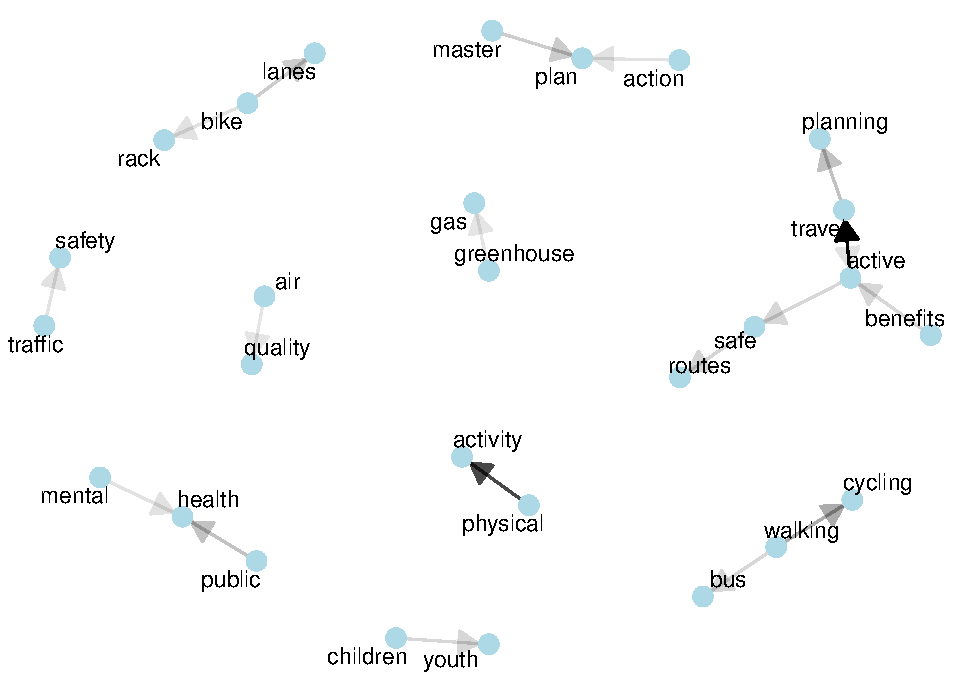
\includegraphics[width=1\linewidth]{AST-Framing-Ontario_files/figure-latex/city-visual-1} 

}

\caption{Most common bigrams found in the municipal or regional government documents.}\label{fig:city-visual}
\end{figure}

\begin{figure}

{\centering 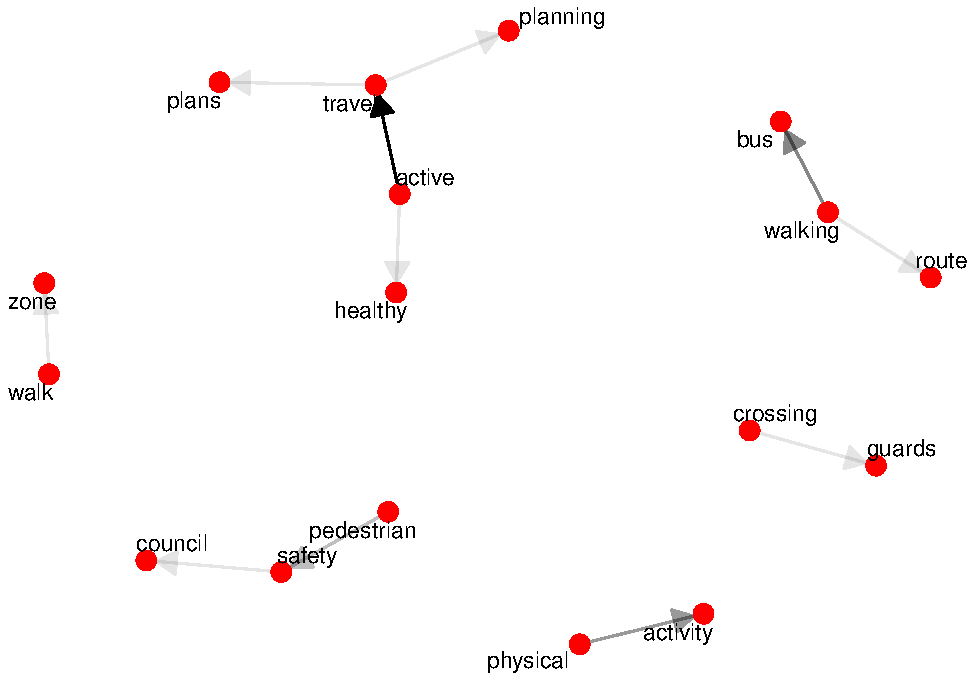
\includegraphics[width=1\linewidth]{AST-Framing-Ontario_files/figure-latex/consortia-visual-1} 

}

\caption{Most common bigrams found in the transportation consortia documents.}\label{fig:consortia-visual}
\end{figure}

\begin{figure}

{\centering 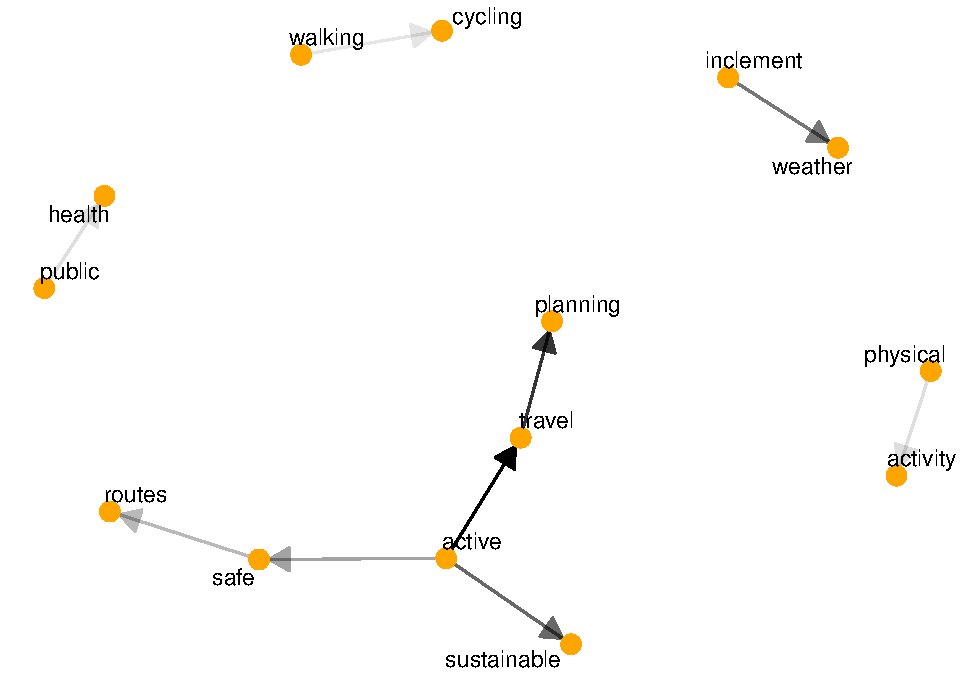
\includegraphics[width=1\linewidth]{AST-Framing-Ontario_files/figure-latex/school-visual-1} 

}

\caption{Most common bigrams found in the school board documents.}\label{fig:school-visual}
\end{figure}

\begin{figure}

{\centering 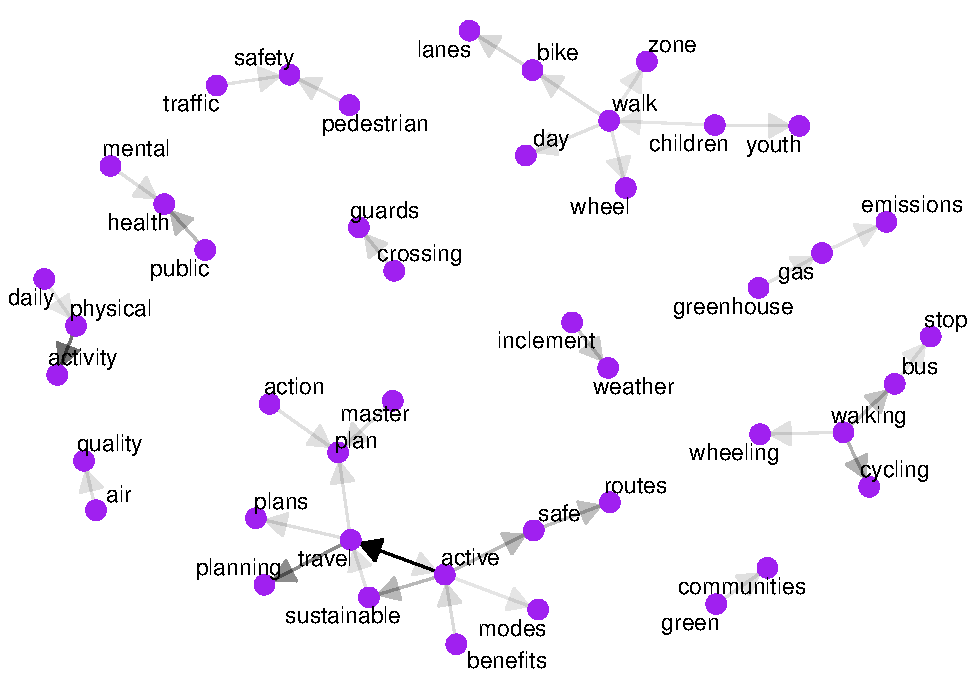
\includegraphics[width=1\linewidth]{AST-Framing-Ontario_files/figure-latex/policy-visual-1} 

}

\caption{Most common bigrams found in all of the policy documents (i.e., school board, municipality, and transportation consortia combined.}\label{fig:policy-visual}
\end{figure}

We combined all of the municipality, school board, and transportation
consortia documents into one ``policy'' corpora. This enabled us to
examine and visualize the most common bigrams found across all of the
STP material in Ontario. Figure \ref{fig:policy-visual} shows all of the
bigrams that occur more than 10 times in the corpora. In addition to the
common bigrams already identified above, we also found \emph{mental
health}, \emph{walk day}, and \emph{green communities} as common pairs
of consecutive words. Overall, policy documents from STP stakeholders
focus on four key areas: i) benefits or impacts of AST; ii) mechanisms
of intervention; iii) concerns or considerations; and iv) supports for
AST.

We analyzed bigrams in the academic corpora separately to make
comparisons with the policy corpora. Figure \ref{fig:academic-visual}
indicates that the academic corpora includes several common bigrams that
were also found in the policy documents including \emph{physical
activity} (n = 1566), which is the top bigram, \emph{traffic safety} (n
= 308), and \emph{safe routes} (n = 268). However, many other factors
relating to AST are identified in the research literature that are not
presented to the public through policy documents. After \emph{physical
activity}, \emph{built environment} (n = 1175), \emph{independent
mobility} (n = 774), and \emph{urban form} (n = 352) are the most
frequent pairs of consecutive words. Academic papers also often discuss
\emph{distance home} (n = 258), \emph{car ownership} (n = 254),
\emph{household income} (n = 254), and \emph{population density} (n =
205), which are factors that have been found to influence AST. It is
evident that many papers investigate gender differences in AST given
that \emph{boys girls} (n = 211) is another common bigram. Finally, the
presence of \emph{statistically significant} among the top bigrams
underscores that researchers aim to identify determinants that are not
due to chance but that likely influence AST. The academic corpora
focuses on a greater range of topics than found in the STP material.

\begin{Shaded}
\begin{Highlighting}[]
\KeywordTok{ggraph}\NormalTok{(academic_bigram_graph, }\DataTypeTok{layout =} \StringTok{"fr"}\NormalTok{) }\OperatorTok{+}
\StringTok{  }\KeywordTok{geom_edge_link}\NormalTok{(}\KeywordTok{aes}\NormalTok{(}\DataTypeTok{edge_alpha =}\NormalTok{ n), }\DataTypeTok{show.legend =} \OtherTok{FALSE}\NormalTok{,}
                 \DataTypeTok{arrow =}\NormalTok{ a, }\DataTypeTok{end_cap =} \KeywordTok{circle}\NormalTok{(.}\DecValTok{07}\NormalTok{, }\StringTok{'inches'}\NormalTok{)) }\OperatorTok{+}
\StringTok{  }\KeywordTok{geom_node_point}\NormalTok{(}\DataTypeTok{color =} \StringTok{"lightgreen"}\NormalTok{, }\DataTypeTok{size =} \DecValTok{4}\NormalTok{) }\OperatorTok{+}
\StringTok{  }\KeywordTok{geom_node_text}\NormalTok{(}\KeywordTok{aes}\NormalTok{(}\DataTypeTok{label =}\NormalTok{ name), }\DataTypeTok{repel =} \OtherTok{TRUE}\NormalTok{) }\OperatorTok{+}\StringTok{ }
\StringTok{  }\KeywordTok{theme_void}\NormalTok{()}
\end{Highlighting}
\end{Shaded}

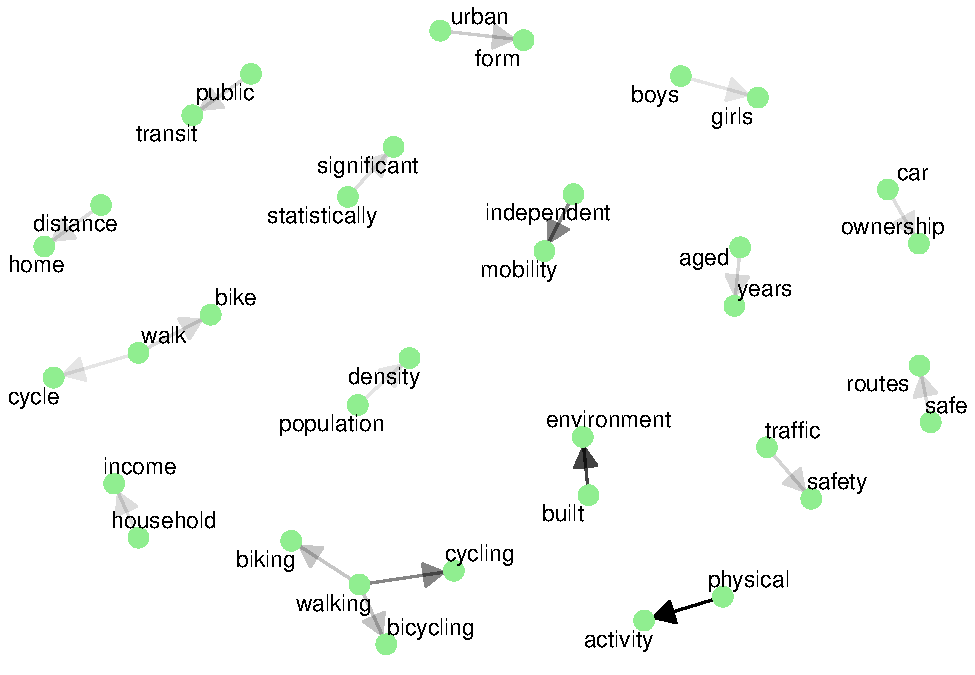
\includegraphics{AST-Framing-Ontario_files/figure-latex/unnamed-chunk-10-1.pdf}

We interpreted the most common bigrams from the policy corpora (see
Figure \ref{fig:policy-visual}), which includes all documents from
municipalities, transportation consortia, and school boards, as the main
ideas that STP stakeholders are focusing on and communicating to the
public about AST. We used the \texttt{kwic} function from the R
\emph{quanteda} package to identify and better understand identify the
context of these key themes.

\begin{table}
\centering
\begin{tabular}[t]{>{}l|l|>{\raggedright\arraybackslash}p{30em}}
\hline
Terms & Stakeholder & Context\\
\hline
\textbf{Physical health} & School Board & ASST not only improves physical and mental health but contributes to a healthier environment and safer streets.\\
\hline
\textbf{Emissions} & Municipality & Encouraging Active Transportation promotes personal health and recreation, helps manage congestion, reduces emissions and supports municipal objectives for efficient land use.\\
\hline
\end{tabular}
\end{table}

\hypertarget{topic-modelling}{%
\subsection{4.3. Topic modelling}\label{topic-modelling}}

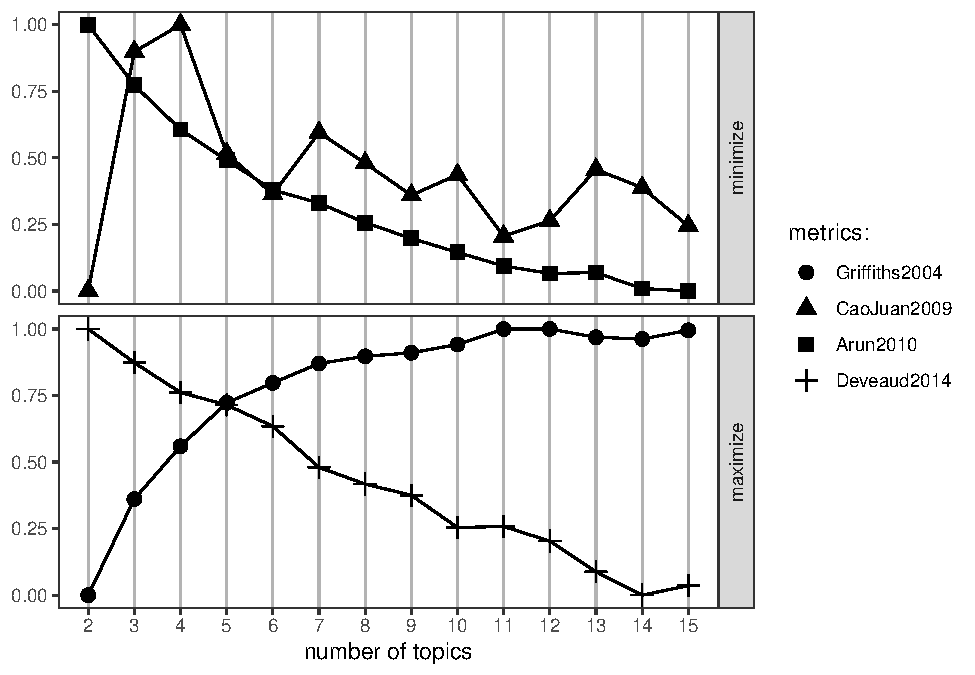
\includegraphics{AST-Framing-Ontario_files/figure-latex/evaluate-lda-1.pdf}
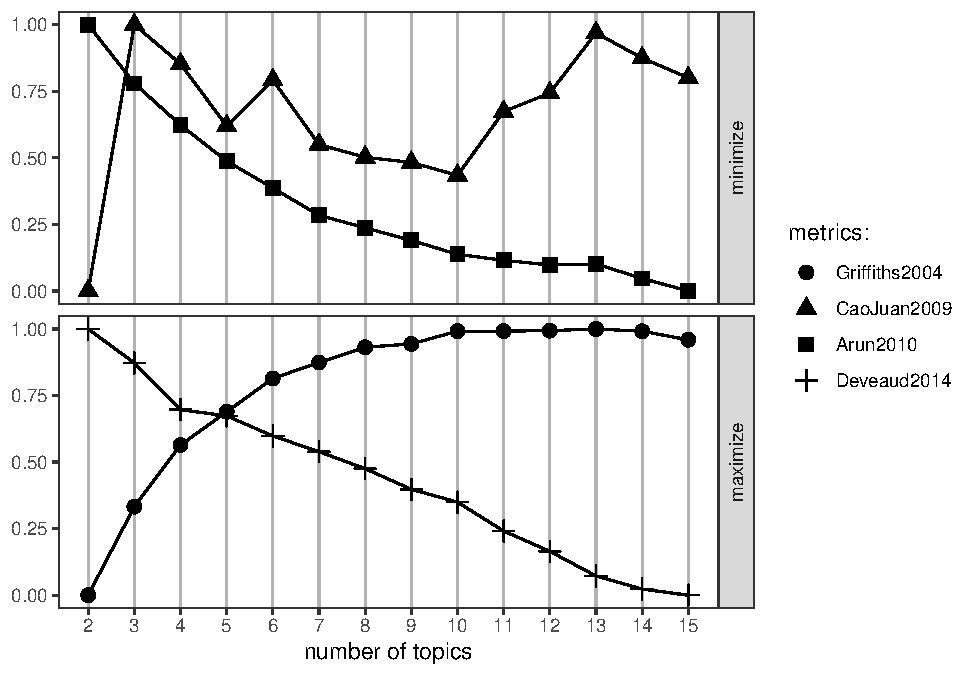
\includegraphics{AST-Framing-Ontario_files/figure-latex/evaluate-lda-2.pdf}
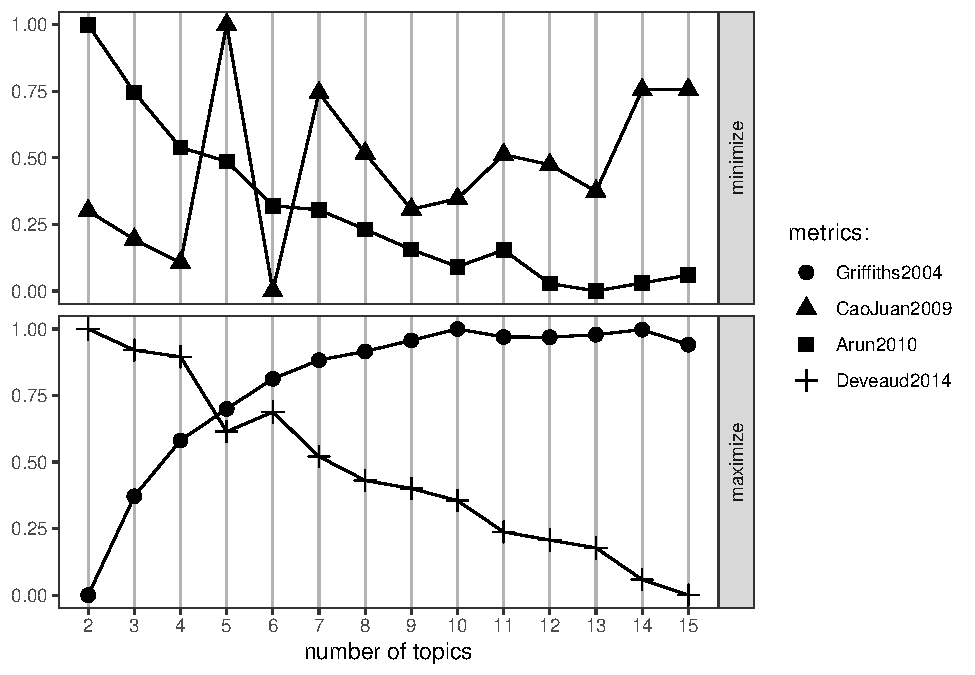
\includegraphics{AST-Framing-Ontario_files/figure-latex/evaluate-lda-3.pdf}
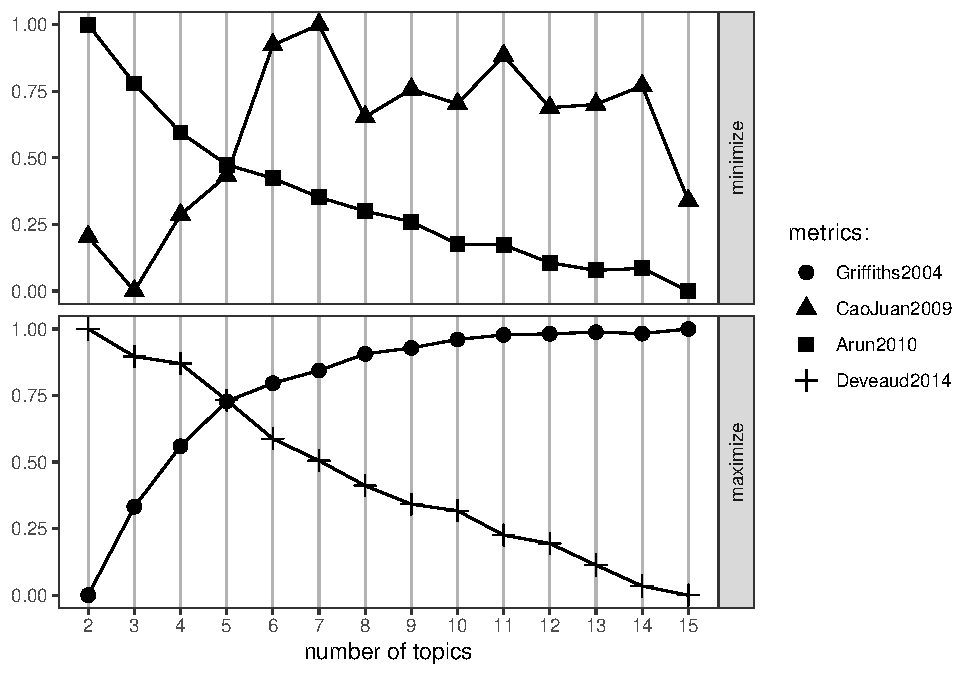
\includegraphics{AST-Framing-Ontario_files/figure-latex/evaluate-lda-4.pdf}

\begin{verbatim}
## final e step document 28
\end{verbatim}

\begin{verbatim}
## final e step document 32
\end{verbatim}

\begin{verbatim}
## final e step document 9
\end{verbatim}

\begin{verbatim}
## final e step document 69
\end{verbatim}

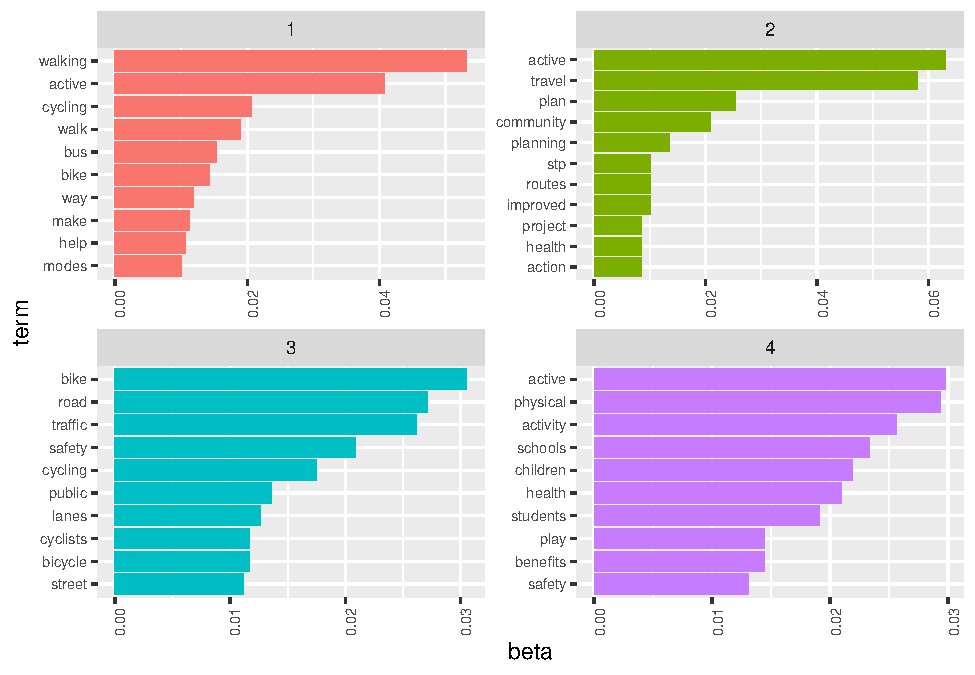
\includegraphics{AST-Framing-Ontario_files/figure-latex/municipal-terms-1.pdf}

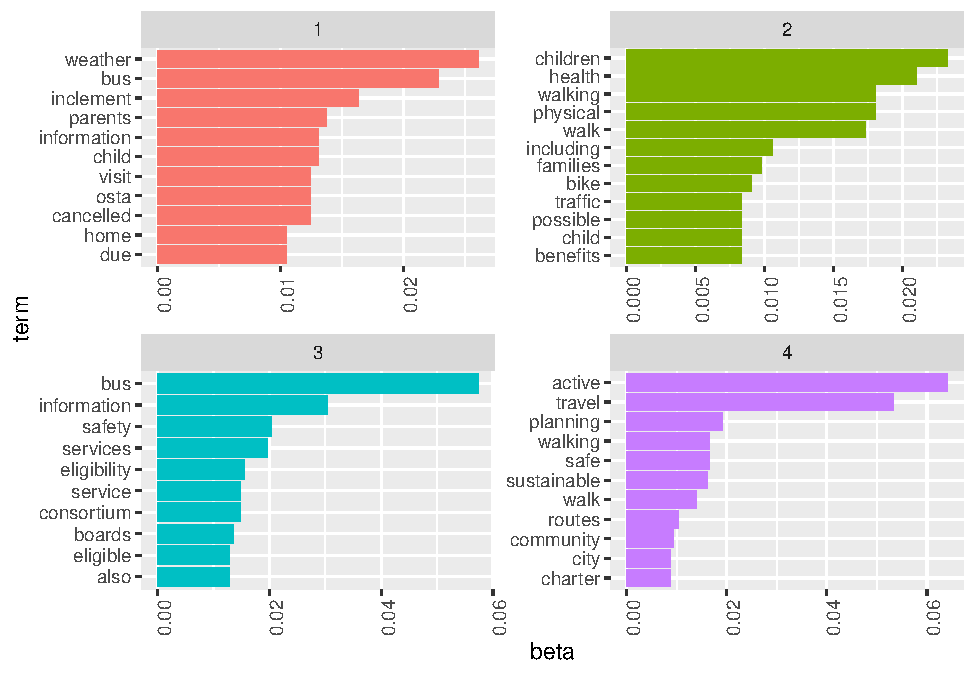
\includegraphics{AST-Framing-Ontario_files/figure-latex/school-terms-1.pdf}

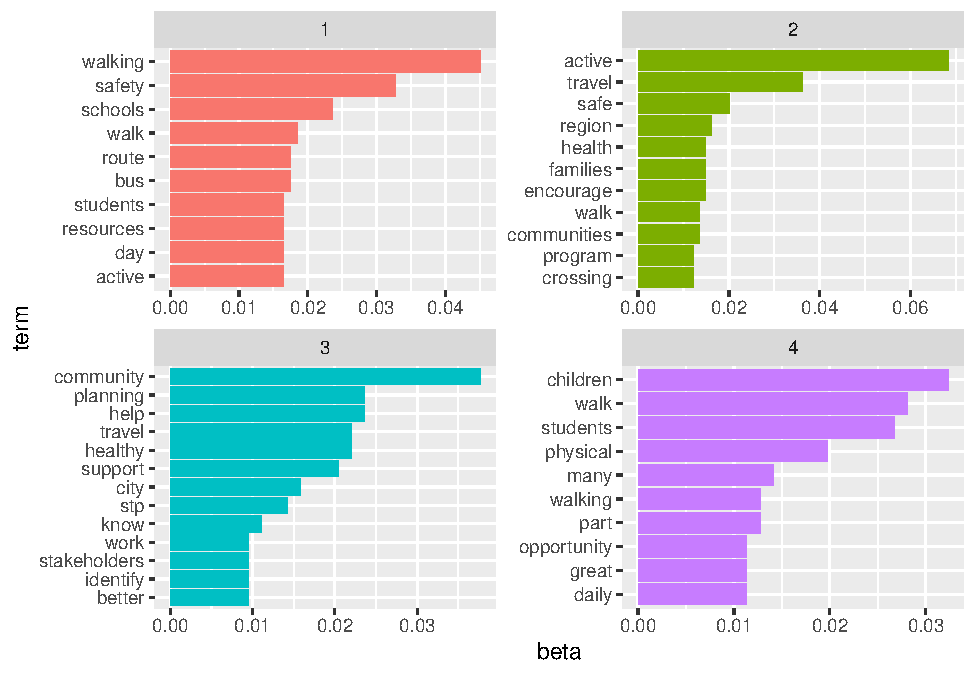
\includegraphics{AST-Framing-Ontario_files/figure-latex/consortia-terms-1.pdf}

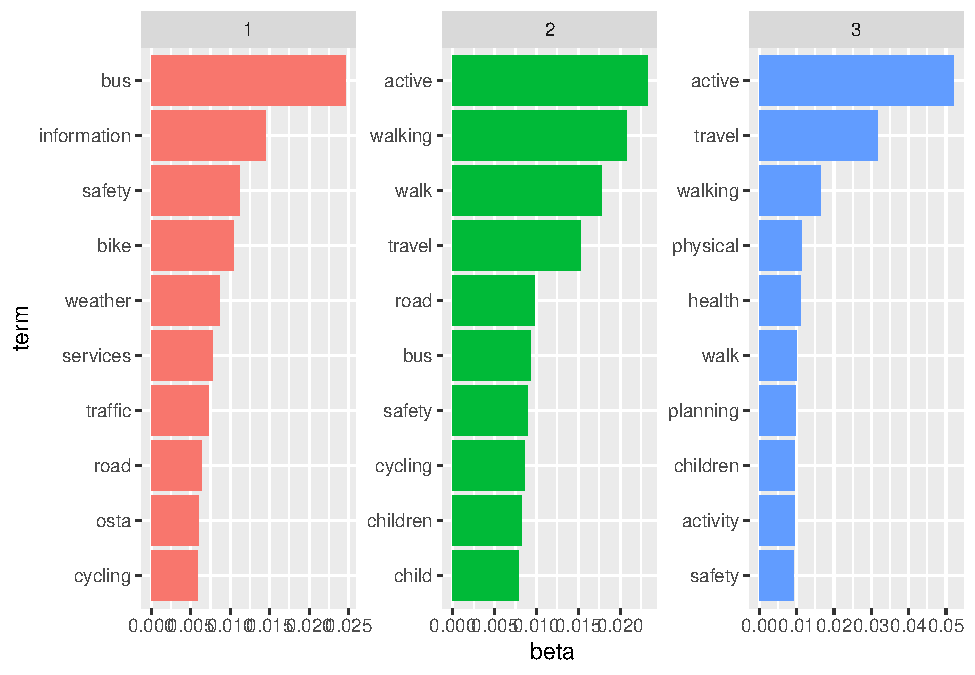
\includegraphics{AST-Framing-Ontario_files/figure-latex/policy-terms-1.pdf}

\begin{Shaded}
\begin{Highlighting}[]
\CommentTok{#municipal_beta <- municipal_topics %>%}
  \CommentTok{#mutate(topic = paste0("topic", topic)) %>%}
  \CommentTok{#pivot_wider(names_from = topic, values_from = beta) %>% }
  \CommentTok{#filter(topic1 > .001 | topic2 > .001) %>%}
  \CommentTok{#mutate(log_ratio = log2(topic2 / topic1))}
\CommentTok{#municipal_beta}
\end{Highlighting}
\end{Shaded}

\begin{Shaded}
\begin{Highlighting}[]
\CommentTok{# Identify topics by document across each corpora}

\NormalTok{municipal_documents <-}\StringTok{ }\KeywordTok{tidy}\NormalTok{(municipal_lda, }\DataTypeTok{matrix =} \StringTok{"gamma"}\NormalTok{)}
\NormalTok{school_documents <-}\StringTok{ }\KeywordTok{tidy}\NormalTok{(school_lda, }\DataTypeTok{matrix =} \StringTok{"gamma"}\NormalTok{)}
\NormalTok{consortia_documents <-}\StringTok{ }\KeywordTok{tidy}\NormalTok{(consortia_lda, }\DataTypeTok{matrix =} \StringTok{"gamma"}\NormalTok{)}
\NormalTok{policy_documents <-}\StringTok{ }\KeywordTok{tidy}\NormalTok{(policy_lda, }\DataTypeTok{matrix =} \StringTok{"gamma"}\NormalTok{)}
\CommentTok{#academic_documents <- tidy(academic_lda, matrix = "gamma")}
\end{Highlighting}
\end{Shaded}

\hypertarget{discussion}{%
\section{5. Discussion}\label{discussion}}

\hypertarget{implications-for-school-travel-planning}{%
\subsection{5.1. Implications for School Travel
Planning}\label{implications-for-school-travel-planning}}

\hypertarget{limitations}{%
\subsection{5.2. Limitations}\label{limitations}}

\hypertarget{conclusion}{%
\section{6.1. Conclusion}\label{conclusion}}

\hypertarget{future-research}{%
\subsection{6.1. Future research}\label{future-research}}

\hypertarget{acknowledgments}{%
\section{Acknowledgments}\label{acknowledgments}}

This research was completed using open software, and the authors wish to
acknowledge the developers of the following \texttt{R} packages:
\texttt{dplyr} ({\textbf{???}}), \texttt{ggraph} ({\textbf{???}}),
\texttt{ggplot2} ({\textbf{???}}), \texttt{igraph} ({\textbf{???}}),
\texttt{pdftools} ({\textbf{???}}), \texttt{readr} ({\textbf{???}}),
\texttt{reshape2} ({\textbf{???}}), \texttt{stringr} ({\textbf{???}}),
\texttt{text2vec} ({\textbf{???}}), \texttt{textdata} ({\textbf{???}}),
\texttt{tidyr} ({\textbf{???}}), \texttt{tidytext} ({\textbf{???}}),
\texttt{tm} ({\textbf{???}}), \texttt{tools} ({\textbf{???}}),
\texttt{topicmodels} ({\textbf{???}}), \texttt{widyr} ({\textbf{???}}),
\texttt{word2vec} ({\textbf{???}}), \texttt{wordcloud} ({\textbf{???}}),
\texttt{DiagrammeR} ({\textbf{???}}), and \texttt{kableextra}
({\textbf{???}}).

\hypertarget{references}{%
\section{References}\label{references}}


\end{document}


